\section{LLVM 中如何实现这个算法}


\begin{frame}
    \frametitle{TL; DR}

    算法主体主要实现在 lib/CodeGen/MachineBlockPlacement.cpp

    \vspace{1.5em}

    其中分支概率等信息来源于 Block\{Frequency, ProbabilityInfo\}

    \vspace{1.5em}

    各个 Target 需要实现 \{ analyze, insert, remove \}Branch等虚函数,RISC-V在 5 年前,D40808\cite{llvmriscvimplbranchanalysis2017}实现;两年前,D84833包含了一个间接分支实现 \cite{llvmriscvimplindirect2020}
    \begin{table}
        \begin{tabular}{ccc}
            \toprule
            功能   & 实现                    & 源代码位置                                                                         \\
            \midrule
            边权   & BlockFrequency        & \cite{llvmblockfreqinfoimpl2022}                                              \\
            块放置  & MachineBlockPlacement & buildCFGChains()\cite{llvmmachineblockplacement2022}                          \\
            块对齐  & MachineBlockPlacement & alignBlocks()\cite{llvmmachineblockplacement2022}                             \\
            分支分析 & RISCVInstrInfo        & analyzeBranch()\cite{llvmriscvinstrinfo2022, llvmriscvimplbranchanalysis2017} \\
            \bottomrule
        \end{tabular}
        \caption{各个功能的实现情况和所在的位置}
    \end{table}

\end{frame}

\begin{frame}
    \frametitle{最开始的布局优化Pass - CodePlacementOptPass}

    2009 年10月,此时 LLVM 大仓库还只有 clang、compiler-rt、llvm.这时 LLVM 的布局优化 Pass 还没有基于 Macine-IR,CodePlacementOptPass ($O(n^2)$) \cite{llvmcodeplacementopt2009}将一些循环尾部的,无条件跳转到循环首部(back-edges)的块,移动到循环的开头.

    \begin{figure}
        \centering
        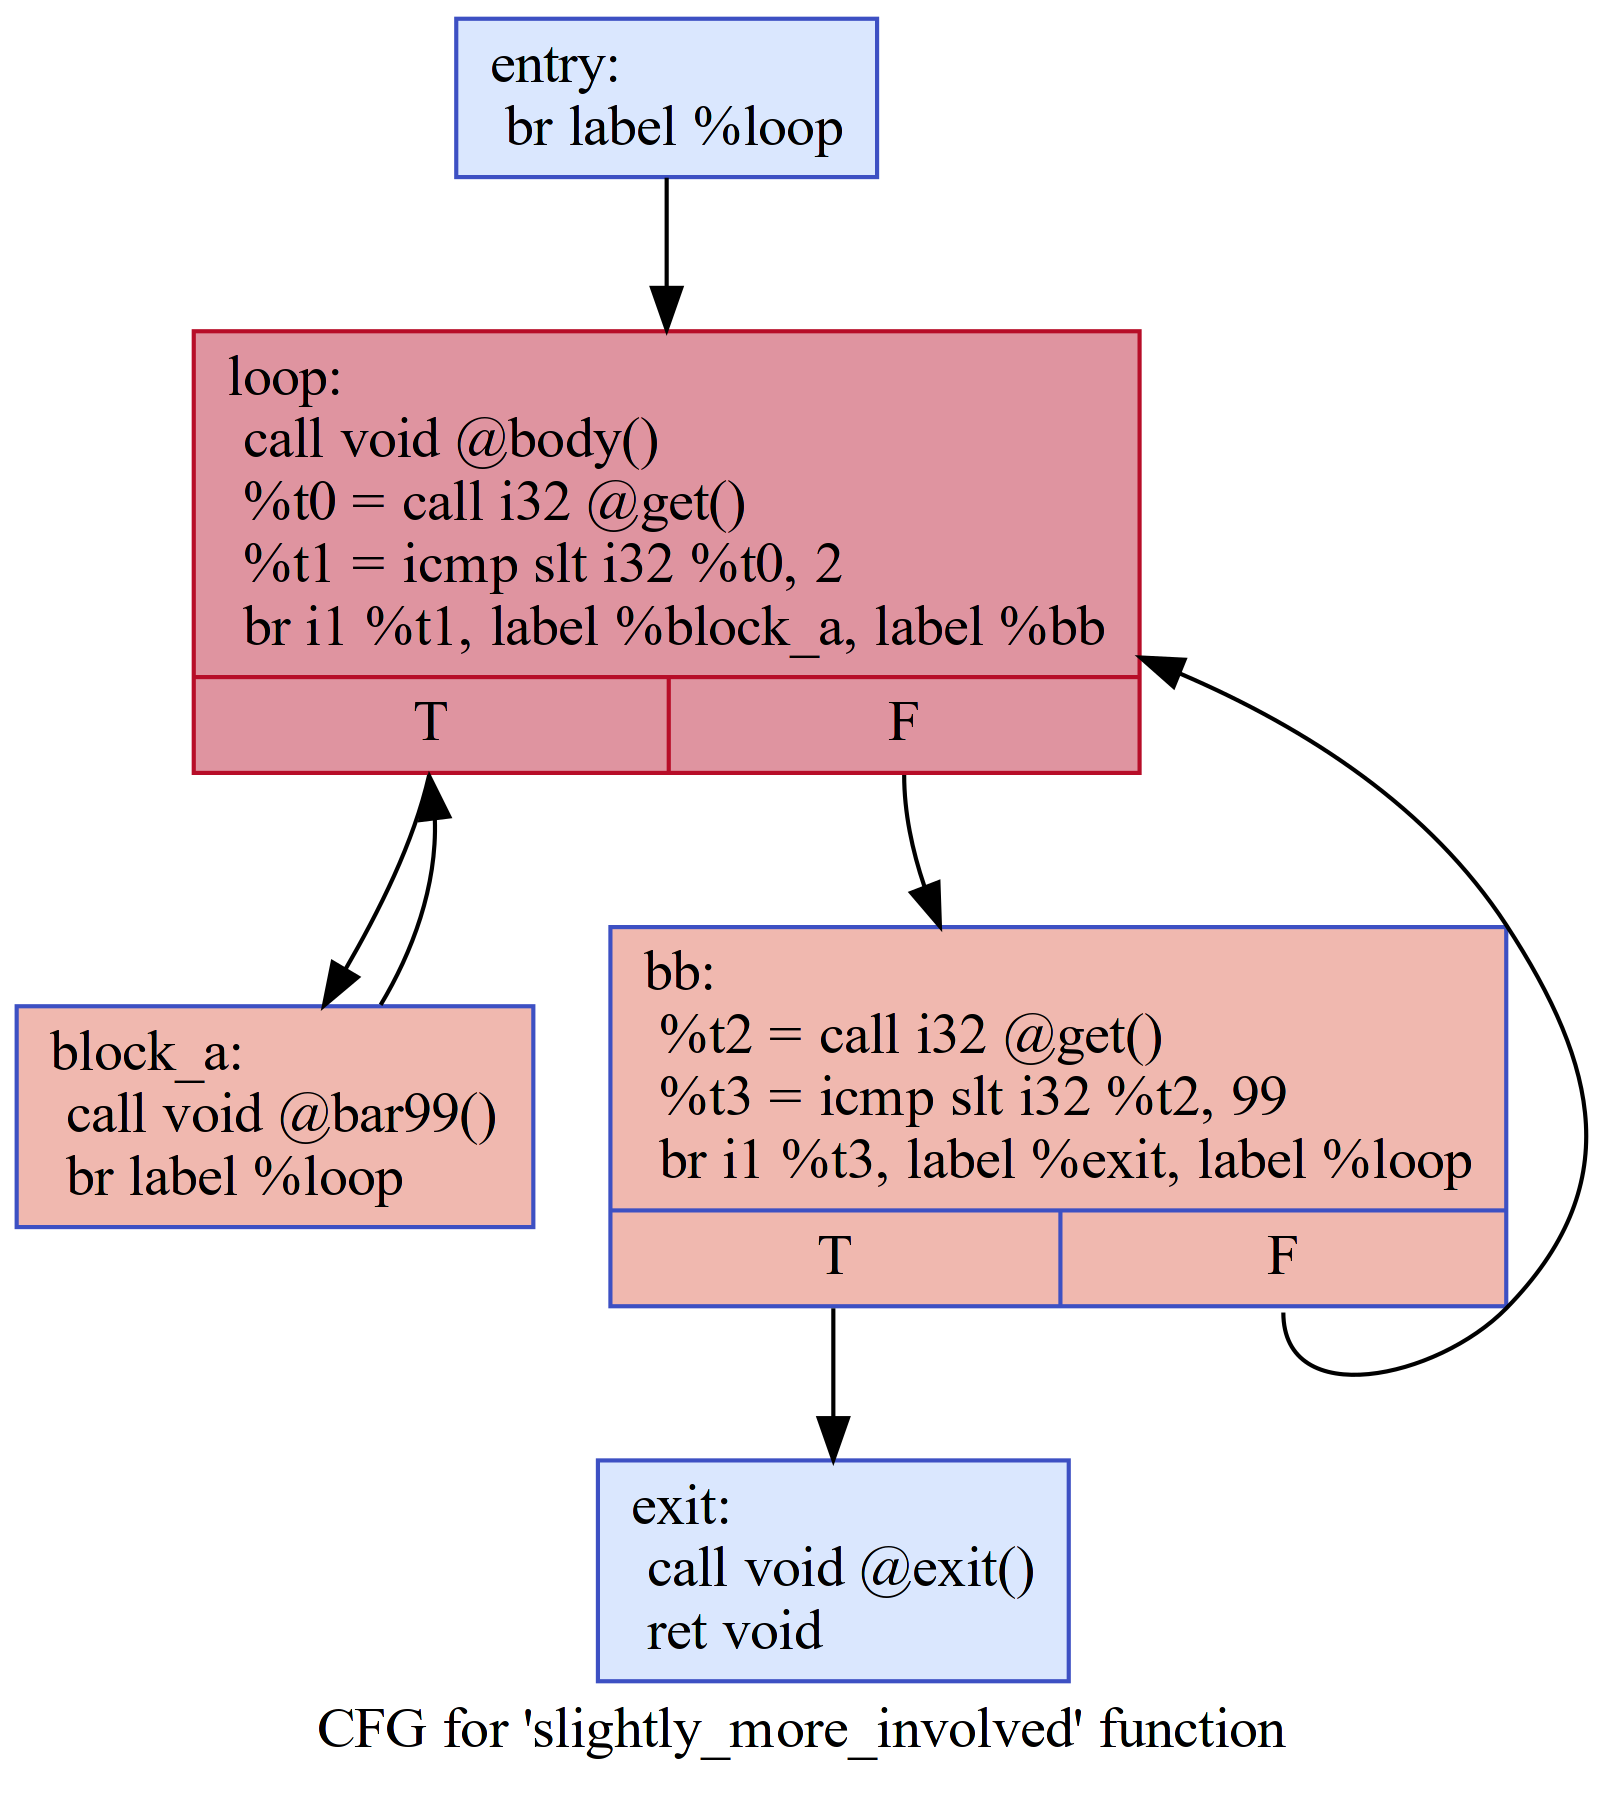
\includegraphics[width=0.25\textwidth]{images/slightly_more_involved.png}
        \caption{block\_a可以被提到循环的开头}
    \end{figure}

\end{frame}


\begin{frame}
    \frametitle{Branch Probability Basic Block Placement - Pettis-Hansen}

    2011年,基于分支概率的基本块被引入,Branch Probability Basic Block Placement 第一次全名出现在了LLVM中 \cite{llvmmachineblockplacementintro2011}.这个算法先把所有的 BB 形成若干链,然后基于强连通分量合并这些链,形成最终的layout.

    然而这个算法很快被废弃,在11月完成了现在所看的版本的雏形,同时也是上面介绍给大家的版本 \cite{llvmmachineblockplacementimporve2011-1, llvmmachineblockplacementimporve2011-2}. 这个版本的算法递归地从循环中构建链,同时尽量保证 CFG 的拓扑序正确.


    

\end{frame}

\begin{frame}
    \frametitle{LLVM 对 Pettis-Hansen 算法的改进}

    2021年12月,MachineBlockPlacement 的基本功能有了新的改进.D113424\cite{llvmexttspbbl2021} 引入一个方案,来优化已经完成链剖分之后的,生成最终的代码布局的过程.

    \begin{figure}
        \begin{tikzpicture}[>=latex',line join=bevel,scale=0.6]
    \pgfsetlinewidth{1bp}
    %%
    \begin{scope}
        \pgfsetstrokecolor{black}
        \definecolor{strokecol}{rgb}{0.0,0.0,0.0};
        \pgfsetstrokecolor{strokecol}
        \draw (8.0bp,8.0bp) -- (8.0bp,227.0bp) -- (78.0bp,227.0bp) -- (78.0bp,8.0bp) -- cycle;
        \draw (43.0bp,215.5bp) node {Chain X};
    \end{scope}
    \begin{scope}
        \pgfsetstrokecolor{black}
        \definecolor{strokecol}{rgb}{0.0,0.0,0.0};
        \pgfsetstrokecolor{strokecol}
        \draw (86.0bp,152.0bp) -- (86.0bp,227.0bp) -- (156.0bp,227.0bp) -- (156.0bp,152.0bp) -- cycle;
        \draw (121.0bp,215.5bp) node {Chain Y};
    \end{scope}
    \pgfsetcolor{black}
    % Edge: X1 -> X2
    \draw [->] (43.0bp,159.7bp) .. controls (43.0bp,151.98bp) and (43.0bp,142.71bp)  .. (43.0bp,124.1bp);
    % Edge: X2 -> X3
    \draw [->] (43.0bp,87.697bp) .. controls (43.0bp,79.983bp) and (43.0bp,70.712bp)  .. (43.0bp,52.104bp);
    % Node: X1
    \begin{scope}
        \definecolor{strokecol}{rgb}{0.68,0.85,0.9};
        \pgfsetstrokecolor{strokecol}
        \definecolor{fillcol}{rgb}{0.68,0.85,0.9};
        \pgfsetfillcolor{fillcol}
        \filldraw [opacity=1] (43.0bp,178.0bp) ellipse (27.0bp and 18.0bp);
        \definecolor{strokecol}{rgb}{0.0,0.0,0.0};
        \pgfsetstrokecolor{strokecol}
        \draw (43.0bp,178.0bp) node {X1};
    \end{scope}
    % Node: X2
    \begin{scope}
        \definecolor{strokecol}{rgb}{0.68,0.85,0.9};
        \pgfsetstrokecolor{strokecol}
        \definecolor{fillcol}{rgb}{0.68,0.85,0.9};
        \pgfsetfillcolor{fillcol}
        \filldraw [opacity=1] (43.0bp,106.0bp) ellipse (27.0bp and 18.0bp);
        \definecolor{strokecol}{rgb}{0.0,0.0,0.0};
        \pgfsetstrokecolor{strokecol}
        \draw (43.0bp,106.0bp) node {X2};
    \end{scope}
    % Node: X3
    \begin{scope}
        \definecolor{strokecol}{rgb}{0.68,0.85,0.9};
        \pgfsetstrokecolor{strokecol}
        \definecolor{fillcol}{rgb}{0.68,0.85,0.9};
        \pgfsetfillcolor{fillcol}
        \filldraw [opacity=1] (43.0bp,34.0bp) ellipse (27.0bp and 18.0bp);
        \definecolor{strokecol}{rgb}{0.0,0.0,0.0};
        \pgfsetstrokecolor{strokecol}
        \draw (43.0bp,34.0bp) node {X3};
    \end{scope}
    % Node: Y
    \begin{scope}
        \definecolor{strokecol}{rgb}{0.68,0.85,0.9};
        \pgfsetstrokecolor{strokecol}
        \definecolor{fillcol}{rgb}{0.68,0.85,0.9};
        \pgfsetfillcolor{fillcol}
        \filldraw [opacity=1] (121.0bp,178.0bp) ellipse (27.0bp and 18.0bp);
        \definecolor{strokecol}{rgb}{0.0,0.0,0.0};
        \pgfsetstrokecolor{strokecol}
        \draw (121.0bp,178.0bp) node {Y};
    \end{scope}
    %
\end{tikzpicture}
        \caption{需要合并的两个Chain示意}
    \end{figure}

\end{frame}

\begin{frame}
    \frametitle{BOLT - Binary optimization and layout tool}

    Facebook 在 2018 年开源了他们的二进制优化工具 -- BOLT\cite{facebook2018bolt, panchenko2019bolt}.这个仓库现在已经合并到 LLVM,可以在对编译后的二进制进行基本的重排,冷热代码分离等工作.

    \begin{figure}
        \centering
        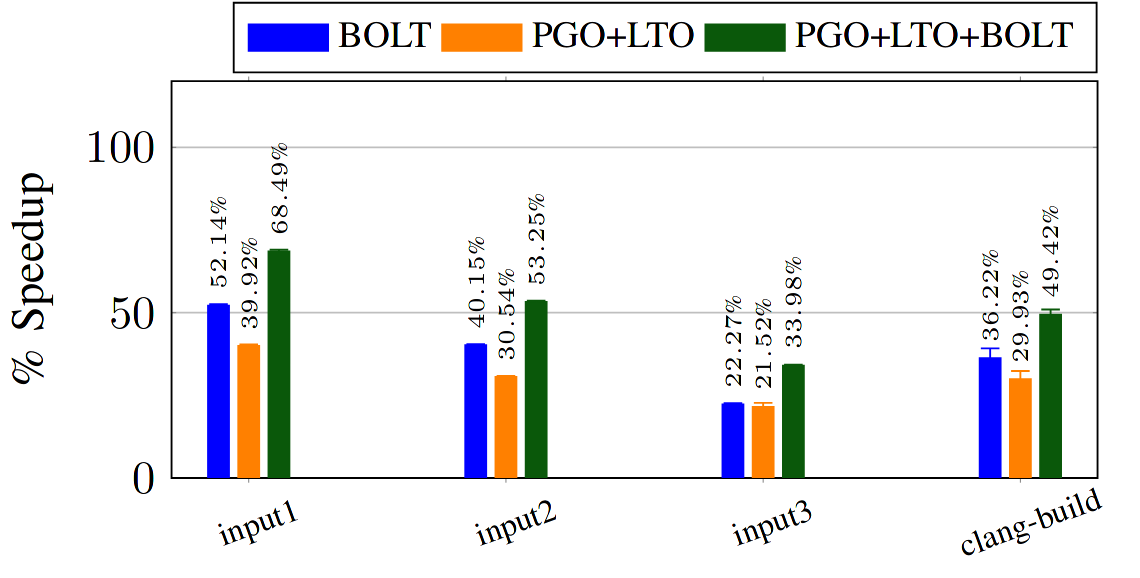
\includegraphics[width=0.6\textwidth]{images/perf_improv_clang.png}
        \caption{优化后的Clang}
    \end{figure}

\end{frame}